\chapter{MIMIC-III}\label{chap:MIMIC}

\section{Introduction}

We carried-out simulations with synthetic patient arrival datasets, and compares the posterior distribution results and prediction rate between Independent Bayes Model (IBM) and Hierarchical Bayes Model (HBM) for-real life data, for the scenarios of common, rare and extremely rare diseases. Sections 3.2 to 3.8 provides background information about the MIMIC-III database. Sections 3.9 gives the result of our analyses. Lastly,  Section 3.10 forms our discussion. 

\section{Source of Data}

For this thesis, datasets from the Medical Information Mart for Intensive Care version 1.4 (MIMIC-III v1.4) database, available on PhysioNet Clinical Databases (\href{https://mimic.physionet.org}{https://mimic.physionet.org}), was used. MIMIC-III is a large, open-access, well maintained database with a collection of de-identified health-related data associated with over 58,000 hospital admissions for 38,645 adults and 7,875 neonates, who was admitted to critical care units of the Beth Israel Deaconess Medical Center (Boston, MA, USA) between the period of June 2001 and October 2012 and is hosted by the Laboratory for Computational Physiology (LCP) at the Massachusetts Institute of Technology (MIT) \citep{johnson2016mimic,Pollard2016mimic,goldberger2000physiobank}. MIMIC-III contains clinical, physiological, and mortality data aggregated from ICU information systems, digital hospital archives, bedside monitors and Social Security Administration Death Master Files. MIMIC-III includes health-related information such as demographics, vital sign measurements, laboratory test results, procedures, medications, caregiver notes, imaging reports, and in and out of hospital mortality registry. Data were collected continuously with non-invasive procedures during routine clinical care and data collection and was blinded from patient and staff, minimising interference with medical routine. Private health information was also de-identified to protect patient privacy \citep{Mark2016}. For example, all dates in the database have been shifted to periods between 2100 to 2200 while conserving seasonal trends. 

\newpara

Access and use of the MIMIC-III database for this thesis have been authorised with a restricted-access to PhysioNet clinical databases and bound by a data use agreement, approved on 9th April 2019. 

\section{ICD-9}

According to the World Health Organisation \citep{WHO2019}, International Statistical Classification of Diseases and Related Health Problems (ICD) is the international standard for clinical diagnosis. ICD defines diseases, disorders, injuries, and other related health conditions in a hierarchical fashion, this allows for storage and access of health-related information internationally, in other words, ICD is the standard for clinical diagnosis. Though there is a subtle variation to the standard as some country adopt different versions. For example, Clinical Modification (ICD-9-CM) is an adaption used in assigning diagnostic in the United States \citep{CDC2019}, and in New Zealand, the Australian Modification (ICD-10-AM) were used \citep{MoH2019}. The version of ICD used for medical diagnosis in the MIMIC dataset is ICD-9, the codes are assigned at the end of the patient’s stay and are used by the hospital to bill for care provided \citep{johnson2016mimic}.

\newpara

\begin{figure}[h]
	\centering
	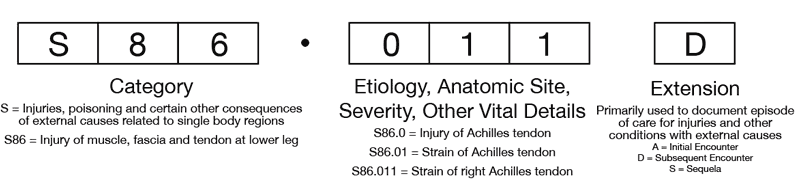
\includegraphics[width=0.7\linewidth]{Figures/icd-10-code}
	\caption{Visualisation of ICD-10 Code Structure, from \cite{Andrus2013}.}
	\label{fig:icd10code}
\end{figure}

As shown in figure~\ref{fig:icd10code}, the first three characters of an ICD codes designate the category of the diagnosis, followed by supplementary information of aetiology (i.e., the cause of condition), anatomic site, severity, or other vital clinical details after a full stop, and may contain an extension used to document episodes of care, this was implemented for ICD 10. For some instances, there may be multiple codes entries for a single condition, like in the case of an Achilles tendon strain, secondary external cause code may be provided along with the primary diagnosis. 

\newpage 

\begin{table}[h!]
	\centering
	\begin{tabular}{|rll|} 
		\hline
		\textbf{Series} & \textbf{ICD-9 Label}  & \textbf{Description}\\ [0.5ex] 
		
		\hline\hline
		\textit{Total}&&\\
		
		1 & -  & International Classification of Diseases, 9th Revision \\ 
		
		\hline    
		\textit{Category lv1}&&\\
		
		1 &001-139  &Infectious And Parasitic Diseases\\
		2 &140-239  &Neoplasms\\
		3 &240-279  &Endocrine, Nutritional And Metabolic Diseases, And \\
		&& Immunity Disorders\\
		...&...&...\\
		17 &800-999  &Injury And Poisoning\\
		18 &V01-V91  &Supplementary Classification Of Factors Influencing \\
		&&Health Status And Contact With Health Services\\
		19 &E000-E999  &Supplementary Classification Of External Causes Of\\
		&& Injury And Poisoning\\
		
		\hline    
		\textit{Category lv2}&\textit{(001-999)}&\\
		
		1 &001-009  &Intestinal Infectious Diseases\\
		2 &010-018  &Tuberculosis\\
		3 &020-027  &Zoonotic Bacterial Diseases\\
		...&...&...\\
		35 &980-989  &Toxic Effects Of Substances Chiefly Nonmedicinal As\\ 
		&&To Source\\
		36 &990-995  &Other And Unspecified Effects Of External Causes\\
		37 &996-999  &Complications Of Surgical And Medical Care, Not \\
		&&Elsewhere Classified\\
		
		\hline    
		\textit{Category lv3}&\textit{(001-999)}&\\
		
		1 &001 &Cholera\\
		2 &002 &Typhoid and paratyphoid fevers\\
		3 &003 &Other salmonella infections\\
		\...&...&...\\
		89&997 &Complications affecting specified body system not \\
		&& elsewhere classified\\
		89&998 &Other complications of procedures not elsewhere \\
		&&classified\\
		89&999 &Complications of medical care not elsewhere classified\\
		
		\hline
		
	\end{tabular}
	\caption{ICD-9 Diagnosis Codes}
	\label{fig:icd10table}
\end{table}

\newpage

ICD 9 categories are coded from 001 to 999, with two extra supplementary class of categories starting with V and E. For example, 001 code for Cholera, and E880 is the code for Accidental fall on or from stairs or steps. Several categories are aggregated to form a larger category, and there are two aggregations which made ICD a three-level hierarchical structure. Following Cholera at level 3, it is aggregated into Intestinal Infectious Diseases for categories from 001 to 009 at level 2, and Infectious and Parasitic Diseases for the categories from 001 to 139 at level 1. Level 1 categories are sometimes referred to as chapters. ICD groupings help to provide a picture of the health situation of the general populations. This information is useful in health care management, and allocation of resources, and other health-related decision-making processes, such as billing of services. Table~\ref{fig:icd10table} provides some examples of ICD codes in different level of ICD categories. There are 632 categories at level 3 of the hierarchy, as those descibed in Table~\ref{fig:icd10table}, there are even finer categories, and national adaptions. ICD-10-CM (usedin USA), for example, has over 70,000 distinct codes \cite{ICD2019}. 

\section{Study Population }

Study inclusion criteria were ICU admission of patients of all age with available documentation of primary ICD-9 diagnosis, excluding supplementary diagnoses (ICD codes start with V or E). Repeated admission to ICU by the same patient were included. The final dataset used contain 50959 uniquely identified Hospital admission event with 38869 uniquely identified patients. 

\section{Study Variables}

Three datasets were merged, including the admissions table, the diagnoses\_icd table and the d\_icd\_diagnoses table. Hospital Admission ID and Subject Id were used to as key identifiers. No demographic information was collected, some event-related information were included, these include Admission time, admission type and admission location. Admission time was converted to admission date. ICD-9 codes used only to contain the first three digits of the full ICD code, the reason for it is that further digits do not reflect any categorical characteristics and will only increase the number of non-significant sub-categories. Supplementary ICD codes that start with V or E were not used, which meant we have ICD codes range from 001 to 999. We defined level 2 and level 3 ICD categories according to the standard ICD-9 definition and created flag/dummy variables for each category. There are 132 unique level 2 ICD categories and 631 unique level 3 ICD categories that were created. Short and long title associated with ICD codes were also included. 

\section{Model}

This section presents the Independent Bayesian Model(IBM) and Hierarchical Bayesian Model(HBM) that is used to calculate posterior distributions. 

\newpara

It is believed that time series prediction are a good prior belief that makes sense, we do not know what the arrival for today will be but we can make an educated guess using our historical records. predictions about the expected daily arrival are used as our prior values, with data for all observed values for the dates prior to the prediction date, using \texttt{predict.hts} Function inside the R environment. Forecast method used is Autoregressive integrated moving average (ARIMA), prediction function used is \texttt{tbats}, and parallel processing is activated to speed up the prediction process. Examples of R-codes used for the time series prediction can be found in Appendix~\ref{htsp}. 

\newpara

For the IBM model, predictions are made with the bottom-up approach by setting argument \texttt{method = "bu"}, the reason for it is that the bottom-up approach makes independent predictions at the leaf level, and does not take into account the hierarchical structure of the data and are suitable for IBM model. In the other hand, predictions for the IBM model are made with the optimal reconciliation approach by setting argument \texttt{method = "comb"}, optimal reconciliation approach reconciles prediction from individual time forecasts from all levels and gives an optimum solutions as the forecast, which meant that the approach takes into account the hierarchical structure of the data, and are suitable for HBM model. However, current optimum solutions will give nonsensical negative predictions. However, these negative solutions are mostly extremely small and close to 0 and are therefore simply converted to 0. So the optimal reconciliation forecasts used for our HBM model are not the actual optimum solution, but the adjusted optimal solution. Non-negativity optimal reconciliation for the \texttt{predict.hts} the function is currently being developed and will be released on CRAN in late July, after the submission date of this thesis. 

\newpara

A Normal(1,0.1) distribution is multiplied with the predicted values to add distribution properties to our prior as our weakly-informative prior. For IBM posterior distributions, posteriors of each category are independently calculated with an IBM model. Whereas for HBM posterior distributions, posterior for each category is calculated with an HBM model that considers all of the levels within the hierarchy. JAGS-codes used to build the IBM and HBM are provided in Appendix~\ref{ibmhbm} and Appendix~\ref{ibmhbm2}. 

\newpara

The likelihood model used for our IBM is:

\begin{equation} \label{ibma8}
\begin{aligned}
y_{i,t} & \sim Poisson(\mu_{i,t}) \\  
log(\mu_{i,t}) & = log(\rho_{i,t}\lambda_{i,t}) \\
\end{aligned}
\end{equation}

Priors for model parameters for our IBM is:

\begin{equation} \label{ibm8b}
\begin{aligned}
\lambda_{i,t} & \sim Normal(\mu_{i,t},\sigma_{i,t}) T_{[\lambda>0]}\\
\end{aligned}
\end{equation}

Hyper-priors for model parameters for our IBM is:

\begin{equation} \label{ibmc8}
\begin{aligned}
\mu_{i,t} & \sim Normal(1,0.1)\\
\sigma^2_{i,t} &\sim Normal(0.1,0.1)\\
\end{aligned}
\end{equation}

The likelihood model used for our HBM is also:

\begin{equation} \label{hbma8}
\begin{aligned}
y_{i,t} & \sim Poisson(\mu_{i,t}) \\  
log(\mu_{i,t}) & = log(\rho_{i,t}\lambda_{i,t}) \\
\end{aligned}
\end{equation}

But $\lambda_{i,t}$ used for different levels of the hierarchy are interconnected with priors and hyper-priors and hyper-hyper priors and so on, that captures the hierarchical structure of our ICD-9 categories.

\newpara

For level 0 category(total):

\begin{equation} \label{hbm8b}
\begin{aligned}
\lambda_{(lv0)i,t} & \sim Normal(\mu_{(lv0)i,t},\sigma_{(lv0)i,t}) T_{[\lambda>0]}\\
\mu_{(lv0)i,t} & \sim Normal(1,0.1)\\
\sigma^2_{(lv0)i,t} &\sim Normal(0.1,0.1)\\
\end{aligned}
\end{equation}

For level 1 categories:

\begin{equation} \label{hbm8b}
\begin{aligned}
\lambda_{(lv1)i,t} & \sim Normal(\mu_{(lv1)i,t},\sigma_{(lv1)i,t}) T_{[\lambda>0]}\\
\mu_{(lv1)i,t} & \sim Normal(mu_{(lv0)i,t},0.1)\\
\sigma^2_{(lv1)i,t} &\sim Normal(0.1,0.1)\\
\end{aligned}
\end{equation}

For level 2 categories:

\begin{equation} \label{hbm8b}
\begin{aligned}
\lambda_{(lv2)i,t} & \sim Normal(\mu_{(lv2)i,t},\sigma_{(lv2)i,t}) T_{[\lambda>0]}\\
\mu_{(lv2)i,t} & \sim Normal(\mu_{(lv1)i,t},0.1)\\
\sigma^2_{(lv2)i,t} &\sim Normal(0.1,0.1)\\
\end{aligned}
\end{equation}

For level 3 (leaf-level) categories:

\begin{equation} \label{hbm8b}
\begin{aligned}
\lambda_{(lv3)i,t} & \sim Normal(\mu_{(lv3)i,t},\sigma_{(lv3)i,t}) T_{[\lambda>0]}\\
\mu_{(lv3)i,t} & \sim Normal(\mu_{(lv2)i,t},0.1)\\
\sigma^2_{(lv3)i,t} &\sim Normal(0.1,0.1)\\
\end{aligned}
\end{equation}


\section{Anomaly} 

The date of 10 November 2190 is set up to be the default date for anomalies additions, therefore, for yearly data anomaly is added on the year of 2190, for monthly data the anomaly is added on 2090Nov, and so on. Due to limitations in sample size and complexity of the ICD-9 hierarchy, it is decided that the time period that we would use is yearly periods between years of 2100 to 2290, the mimic-3 dataset provides an average of 500 arrivals per year.

\newpara

We are interested in how the anomaly detection rates of Independent Bayesian Model (IBM) and Hierarchical Bayesian Model(HBM) will perform for arrivals of common, rare and extremely rare disease diagnoses. \textbf{Common} disease refers to a disease that public hospitals will likely to always encounter in a time period, in our case we decided to choose category 410, which codes for Acute myocardial infarction, commonly known as a heart attack. There are 3307 cases of Acute myocardial infarction in the MIMIC-III data, making it one of the largest category. Considering the pre-perturbation time period used in MIMIC-III is actually a 12 year period. We can suggest that Acute myocardial infarction as a common disease that the ICU department almost sees daily. \textbf{Rare} disease refers to a disease that public hospitals will unlikely to encounter in a time period, in our case we decided to choose category 415, which codes for Acute pulmonary heart disease, also known as cor pulmonale, is the enlargement and failure of the right ventricle of the heart as a response to increased vascular resistance (such as from pulmonic stenosis) or high blood pressure in the lungs.\citep{MedlinePlus2019}. There are 373 cases of Acute pulmonary heart disease in the MIMIC-III data,  considering the pre-perturbation time period of MIMIC-III is actually a 12 year period, we can suggest that Acute myocardial infarction as a rare disease that the ICU department almost sees monthly. \textbf{Extremely rare} disease refers to a disease that public hospitals will extremely unlikely to encounter in a time period, in our case we decided to choose category 452, which codes for Portal vein thrombosis, it is blockage or narrowing of the portal vein by a blood clot \citep{MSD2019}. There are only 12 cases of Acute pulmonary heart disease in the MIMIC-III data,  considering the pre-perturbation time period of MIMIC-III is actually a 12 year period, we can suggest that Acute myocardial infarction as an extremely rare disease that the ICU department are lucky to see more than once per year. 

\newpara

Three abnormal yearly observations are created to test anomaly detection of the three scenarios when there is definitely anomaly (we added anomaly) present at the lowest level of the hierarchy. Due to the aggregation constraint, the addition of anomaly at the lowest level of the hierarchy will result in the addition of the same number of anomalies to its parent and ancestors. This has an effect on the detection rate in all levels of the hierarchy that relates to the specific category. If the observation is 0, a default anomaly of 1 is added. 

\newpara

%\begin{figure}
%    
%    \caption{Addition of 100\% anomaly to common, rare and extremely rare diseases. }
%    \label{fig:addano}
%\end{figure} 

Overall we are looking at four scenarios. Scenario 1 is the anomaly detection rate of common, rare and extremely rare disease categories of the observed data, without the addition of an anomaly. Scenario 2 is the anomaly detection rate of common disease categories of the observed data, with an addition 100\% anomaly at the lowest hierarchy level. Scenario 3 is the anomaly detection rate of rare disease categories of the observed data, with an addition 100\% anomaly at the lowest hierarchy level. Lastly, in scenario 4, we look at the anomaly detection rate of extremely rare disease categories of the observed data, with an addition 100\% anomaly at the lowest hierarchy level. 

\section{Statistical Analyses}

A DIC comparisons table was first used to compare the difference in DIC distributions of Independent Bayesian Model (IBM) and Hierarchical Bayesian Model (HBM). Posterior distributions of our categories of interest for original and anomaly data are then provided in tables and density plots. Lastly, signals of the anomaly are visualised with a heat-map. SAS version 9.4 \citep{SAS} was used during the data cleaning process, and analyses were performed with R version 3.3.2 \citep{R} in the R Studio environment Version 1.1.463 \citep{Rstudio}. An overview of functions created and models built in this thesis is provided in the Appendix. The full collection of R, JAGS, and SAS codes used to synthesise datasets, clean and merge datasets, run the simulation, and draw table and plots and are available on GitHub repository
\href{https://github.com/jungxue/research-masters-Jung}{https://github.com/jungxue/research-masters-Jung}.

%=============================== Results =====================================

\newpage

\section{Results}

%----------------------------- DIC ----------------------------------

\begin{table}[!h]
	\centering
	\begin{tabular}{rrrrrrrr}
		\hline
		& Min. & 1st Qu. & Median & Mean & 3rd Qu. & Max. & NA's \\ 
		\hline
		No amomaly & -5.635 & -0.443 & -0.004 & 0.095 & 0.494 & 9.212 & 109 \\ 
		410 & -5.579 & -0.416 & 0.005 & 0.118 & 0.547 & 6.933 & 109 \\ 
		415 & -7.660 & -0.438 & -0.010 & -0.007 & 0.444 & 8.195 & 109 \\ 
		452 & -6.540 & -0.466 & -0.002 & 0.048 & 0.496 & 7.628 & 109 \\ 
		\hline
	\end{tabular}
	\caption{DIC comparisons for Independent Bayesian Model and Hierarchical Bayesian model for no anomaly, and anomaly added for common, rare and extremely rare diseases} 
	\label{tab:dicmimic}
\end{table}

\newpara

Table~\ref{tab:dicmimic} gives the comparison of DIC distributions of Independent Bayesian Model (IBM) and Hierarchical Bayesian Model (HBM) for no anomaly, and anomaly added for common, rare and extremely rare diseases. It is tough to tell whether or not HBM perform better than IBM, because the negative signal is very hard to detect, and the mean and median value is very close to 0. Multiple samples of DIC are also not feasible as sampling process took a very long time. Conclusions about goodness-of-fit performance between IBM and HBM can not be made. 



%----------------------------- Posteriors ----------------------------------

\newpage

\begin{table}[!t]
	\centering
	\begin{tabular}{rrrrrrrr}
		\hline
		& mean & sd & 2.5\% & 50\% & 97.5\% & Rhat & n.eff \\ 
		\hline
		total & 526.647 & 22.818 & 482.137 & 526.444 & 573.014 & 1.000 & 2912.000 \\ 
		390-459 & 195.270 & 13.662 & 169.633 & 194.978 & 222.341 & 1.000 & 3000.000 \\ 
		410-414 & 78.372 & 8.798 & 62.315 & 78.048 & 95.974 & 1.000 & 2888.000 \\ 
		415-417 & 3.240 & 1.815 & 0.715 & 2.917 & 7.654 & 1.000 & 2415.000 \\ 
		451-459 & 6.412 & 2.555 & 2.477 & 6.048 & 12.171 & 1.000 & 2191.000 \\ 
		410 & 37.218 & 6.211 & 26.305 & 36.663 & 50.562 & 1.000 & 2879.000 \\ 
		415 & 3.293 & 1.833 & 0.800 & 2.932 & 7.714 & 1.000 & 1977.000 \\ 
		452 & 0.158 & 0.174 & 0.001 & 0.087 & 0.597 & 1.010 & 445.000 \\ 
		\hline
	\end{tabular}
	\caption{Posterior distributions for ICD 410,415 and 452 and its ancestors, with no added anomalies, and calculated with Independent Bayes Model} 
	\label{tab:postsumnorm.mimic}
\end{table}

\begin{figure}[!h]
	\centering
	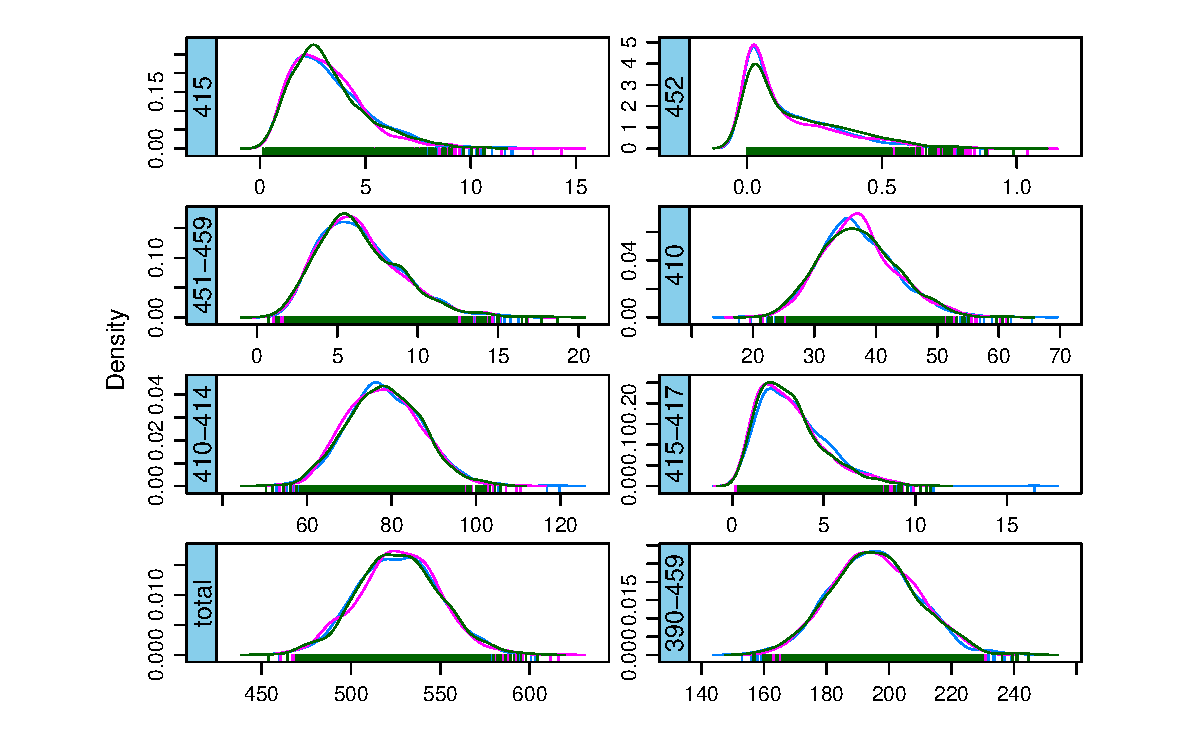
\includegraphics[width=1\linewidth]{../../R-codes/JAGS/plots/mimic/Densitynorm}
	\caption{Posterior distributions for ICD 410,415 and 452 and its ancestors, with no added anomalies, and calculated with Independent Bayes Model}
	\label{fig:densitynorm}
\end{figure}

\newpage

\begin{table}[!t]
	\centering
	\begin{tabular}{rrrrrrrr}
		\hline
		& mean & sd & 2.5\% & 50\% & 97.5\% & Rhat & n.eff \\ 
		\hline
		total & 525.996 & 22.917 & 482.084 & 525.396 & 572.556 & 1.000 & 3000.000 \\ 
		390-459 & 194.540 & 14.077 & 167.744 & 194.275 & 223.211 & 1.000 & 3276.000 \\ 
		410-414 & 78.348 & 8.939 & 62.045 & 77.995 & 96.766 & 1.000 & 3160.000 \\ 
		415-417 & 3.116 & 1.734 & 0.692 & 2.817 & 7.201 & 1.000 & 2174.000 \\ 
		451-459 & 6.288 & 2.344 & 2.516 & 6.053 & 11.522 & 1.010 & 1401.000 \\ 
		410 & 37.678 & 6.166 & 26.738 & 37.342 & 50.959 & 1.000 & 3000.000 \\ 
		415 & 3.319 & 1.949 & 0.703 & 2.954 & 8.441 & 1.000 & 1990.000 \\ 
		452 & 0.150 & 0.169 & 0.001 & 0.082 & 0.607 & 1.050 & 279.000 \\ 
		\hline
	\end{tabular}
	\caption{Posterior distributions for ICD 410,415 and 452 and its ancestors, with no added anomalies, and calculated with Hierarchical Bayes model} 
	\label{tab:postsumnormh.mimic}
\end{table}

\begin{figure}[!h]
	\centering
	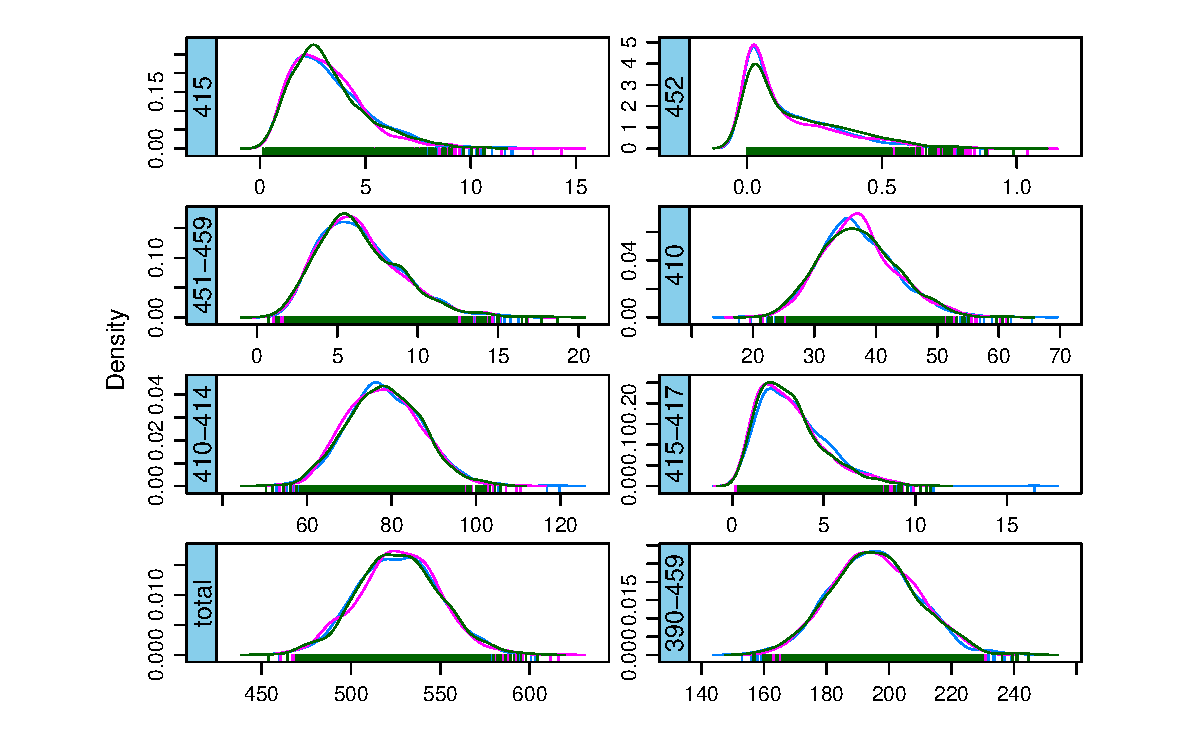
\includegraphics[width=1\linewidth]{../../R-codes/JAGS/plots/mimic/Densitynorm}
	\caption{Posterior distributions for ICD 410,415 and 452 and its ancestors, with no added anomalies, and calculated with Hierarchical Bayes model}
	\label{fig:densitynormh}
\end{figure}

Table~\ref{tab:postsumnorm.mimic} and figure~\ref{fig:densitynorm} shows the posterior for IBM and table~\ref{tab:postsumnormh.mimic} and figure~\ref{fig:densitynormh} shows the posterior for HBM, for ICD 410,415 and 452 and its ancestors, with no added anomalies. There are no obvious differences between the distribution values and distribution shape for IBM and HBM. Distribution for categories at a higher level, and categories with higher mean values tend to approximate to normal, for the case of category 415-417, even though it is at a higher hierarchy level it has a low mean, and the distribution is not normal. 

\newpage%----------------------------------- 410 -------------------------------------------

\begin{table}[!t]
	\centering
	\begin{tabular}{rrrrrrrr}
		\hline
		& mean & sd & 2.5\% & 50\% & 97.5\% & Rhat & n.eff \\ 
		\hline
		total & 563.697 & 23.816 & 518.412 & 563.222 & 612.356 & 1.000 & 3111.000 \\ 
		390-459 & 232.494 & 15.041 & 204.686 & 231.814 & 263.502 & 1.000 & 2905.000 \\ 
		410-414 & 115.402 & 10.918 & 94.819 & 114.956 & 137.937 & 1.000 & 3000.000 \\ 
		410 & 74.630 & 8.617 & 58.748 & 74.137 & 92.840 & 1.000 & 3542.000 \\ 
		\hline
	\end{tabular}
	\caption{Posterior distributions for ICD 410 and its ancestors, with added anomalies, and calculated with independent Bayes model} 
	\label{tab:postsum410.mimic}
\end{table}

\begin{figure}[!h]
	\centering
	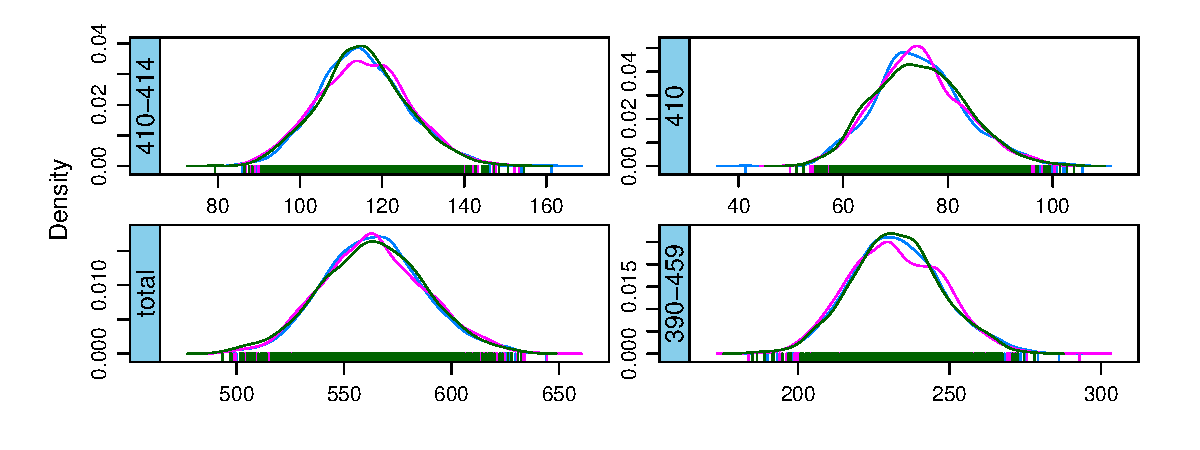
\includegraphics[width=1\linewidth]{../../R-codes/JAGS/plots/mimic/Density410}
	\caption{Posterior distributions for ICD 410 and its ancestors, with added anomalies, and calculated with independent Bayes model}
	\label{fig:density410}
\end{figure}

\newpage%----------------------------------- 410 H -------------------------------------------

\begin{table}[!t]
	\centering
	\begin{tabular}{rrrrrrrr}
		\hline
		& mean & sd & 2.5\% & 50\% & 97.5\% & Rhat & n.eff \\ 
		\hline
		total & 528.324 & 23.296 & 485.619 & 527.677 & 574.402 & 1.000 & 2835.000 \\ 
		390-459 & 197.765 & 13.976 & 171.717 & 197.386 & 225.945 & 1.000 & 3014.000 \\ 
		410-414 & 78.351 & 8.886 & 62.382 & 77.809 & 96.776 & 1.000 & 2860.000 \\ 
		410 & 37.500 & 6.085 & 26.335 & 37.094 & 49.894 & 1.000 & 3138.000 \\ 
		\hline
	\end{tabular}
	\caption{Posterior distributions for ICD 410 and its ancestors, with added anomalies, and calculated with Hierarchiacl Bayes model} 
	\label{tab:postsum410h.mimic}
\end{table}

\begin{figure}[!h]
	\centering
	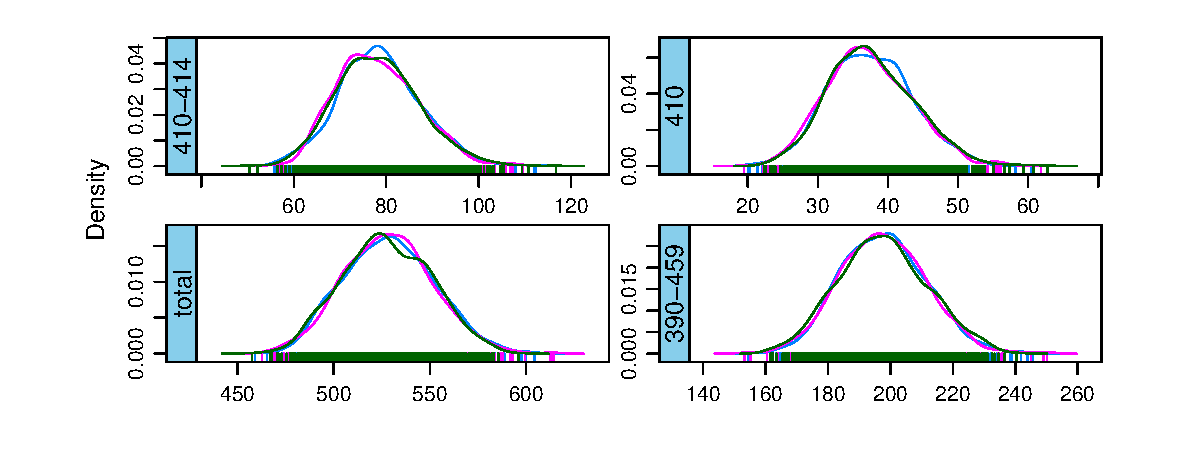
\includegraphics[width=1\linewidth]{../../R-codes/JAGS/plots/mimic/Density410h}
	\caption{Posterior distributions for ICD 410 and its ancestors, with added anomalies, and calculated with Hierarchiacl Bayes model}
	\label{fig:density410h}
\end{figure}

Table~\ref{tab:postsum410.mimic} and figure~\ref{fig:density410} shows the posterior for IBM and table~\ref{tab:postsum410h.mimic} and figure~\ref{fig:density410h} shows the posterior for HBM, for ICD 410 and its ancestors, with added anomalies. There are is an obvious differences (more than double at leaf) between the distribution values and distribution shape for IBM and HBM. 

\newpage%----------------------------------- 415 -------------------------------------------

\begin{table}[!t]
	\centering
	\begin{tabular}{rrrrrrrr}
		\hline
		& mean & sd & 2.5\% & 50\% & 97.5\% & Rhat & n.eff \\ 
		\hline
		total & 528.937 & 23.037 & 484.629 & 528.703 & 574.379 & 1.000 & 2859.000 \\ 
		390-459 & 198.553 & 14.315 & 171.867 & 198.445 & 227.649 & 1.000 & 3000.000 \\ 
		415-417 & 6.364 & 2.494 & 2.470 & 6.059 & 11.999 & 1.000 & 2419.000 \\ 
		415 & 6.436 & 2.571 & 2.373 & 6.117 & 12.070 & 1.000 & 2139.000 \\ 
		\hline
	\end{tabular}
	\caption{Posterior distributions for ICD 415 and its ancestors, with added anomalies, and calculated with independent Bayes model} 
	\label{tab:postsum415.mimic}
\end{table}

\begin{figure}[!h]
	\centering
	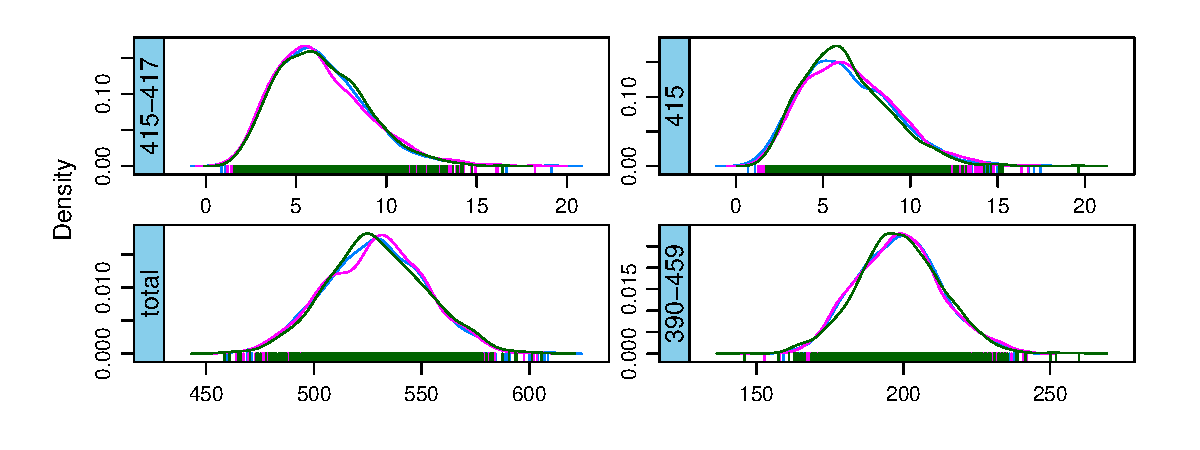
\includegraphics[width=1\linewidth]{../../R-codes/JAGS/plots/mimic/Density415}
	\caption{Posterior distributions for ICD 415 and its ancestors, with added anomalies, and calculated with independent Bayes model}
	\label{fig:density415}
\end{figure}

\newpage%----------------------------------- 415 H -------------------------------------------

\begin{table}[!t]
	\centering
	\begin{tabular}{rrrrrrrr}
		\hline
		& mean & sd & 2.5\% & 50\% & 97.5\% & Rhat & n.eff \\ 
		\hline
		total & 526.519 & 23.086 & 481.720 & 526.254 & 572.876 & 1.000 & 3000.000 \\ 
		390-459 & 195.702 & 13.884 & 169.817 & 195.471 & 223.270 & 1.000 & 3165.000 \\ 
		415-417 & 3.146 & 1.784 & 0.721 & 2.827 & 7.459 & 1.000 & 1876.000 \\ 
		415 & 3.308 & 1.953 & 0.680 & 2.942 & 7.934 & 1.000 & 1730.000 \\ 
		\hline
	\end{tabular}
	\caption{Posterior distributions for ICD 415 and its ancestors, with added anomalies, and calculated with Hierarchical Bayes model} 
	\label{tab:postsum415h.mimic}
\end{table}

\begin{figure}[!h]
	\centering
	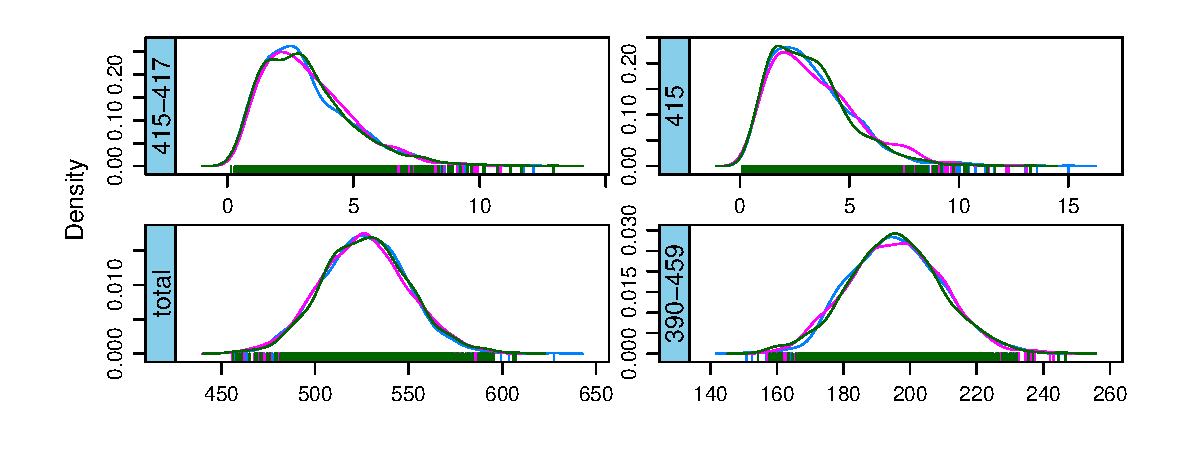
\includegraphics[width=1\linewidth]{../../R-codes/JAGS/plots/mimic/Density415h}
	\caption{Posterior distributions for ICD 415 and its ancestors, with added anomalies, and calculated with Hierarchical Bayes model}
	\label{fig:density415h}
\end{figure}

Table~\ref{tab:postsum415.mimic} and figure~\ref{fig:density415} shows the posterior for IBM and table~\ref{tab:postsum415h.mimic} and figure~\ref{fig:density415h} shows the posterior for HBM, for ICD 415 and its ancestors, with added anomalies. There are is an obvious differences (almost double at leaf) between the distribution values and distribution shape for IBM and HBM.

\newpage%----------------------------------- 452 -------------------------------------------

\begin{table}[!t]
	\centering
	\begin{tabular}{rrrrrrrr}
		\hline
		& mean & sd & 2.5\% & 50\% & 97.5\% & Rhat & n.eff \\ 
		\hline
		total & 526.983 & 23.297 & 480.980 & 526.758 & 573.138 & 1.000 & 3114.000 \\ 
		390-459 & 196.224 & 13.951 & 169.986 & 195.689 & 224.270 & 1.000 & 3294.000 \\ 
		451-459 & 7.382 & 2.629 & 3.052 & 7.077 & 13.190 & 1.000 & 2322.000 \\ 
		452 & 0.346 & 0.208 & 0.033 & 0.323 & 0.812 & 1.000 & 517.000 \\ 
		\hline
	\end{tabular}
	\caption{Posterior distributions for ICD 452 and its ancestors, with added anomalies, and calculated with independent Bayes model} 
	\label{tab:postsum452.mimic}
\end{table}

\begin{figure}[!h]
	\centering
	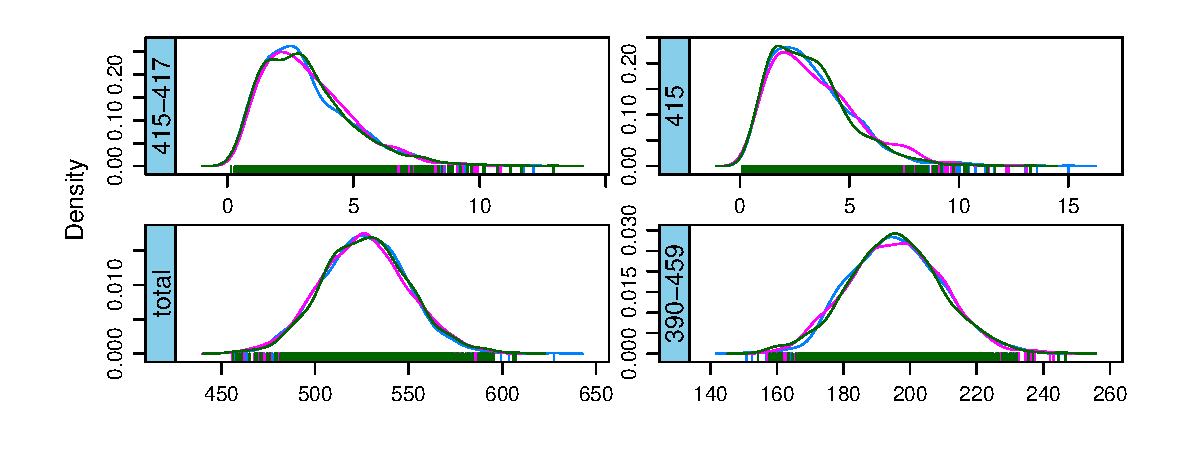
\includegraphics[width=1\linewidth]{../../R-codes/JAGS/plots/mimic/Density415h}
	\caption{Posterior distributions for ICD 452 and its ancestors, with added anomalies, and calculated with independent Bayes model}
	\label{fig:density452}
\end{figure}

\newpage%----------------------------------- 452 H -------------------------------------------

\begin{table}[!t]
	\centering
	\begin{tabular}{rrrrrrrr}
		\hline
		& mean & sd & 2.5\% & 50\% & 97.5\% & Rhat & n.eff \\ 
		\hline
		total & 526.447 & 23.045 & 482.679 & 526.250 & 572.946 & 1.000 & 3061.000 \\ 
		390-459 & 195.096 & 13.618 & 168.448 & 194.678 & 222.373 & 1.000 & 2950.000 \\ 
		451-459 & 7.476 & 2.495 & 3.299 & 7.282 & 13.055 & 1.000 & 1358.000 \\ 
		452 & 0.390 & 0.222 & 0.045 & 0.362 & 0.889 & 1.020 & 342.000 \\ 
		\hline
	\end{tabular}
	\caption{Posterior distributions for ICD 452 and its ancestors, with added anomalies, and calculated with Hierarchical Bayes model} 
	\label{tab:postsum452h.mimic}
\end{table}

\begin{figure}[!h]
	\centering
	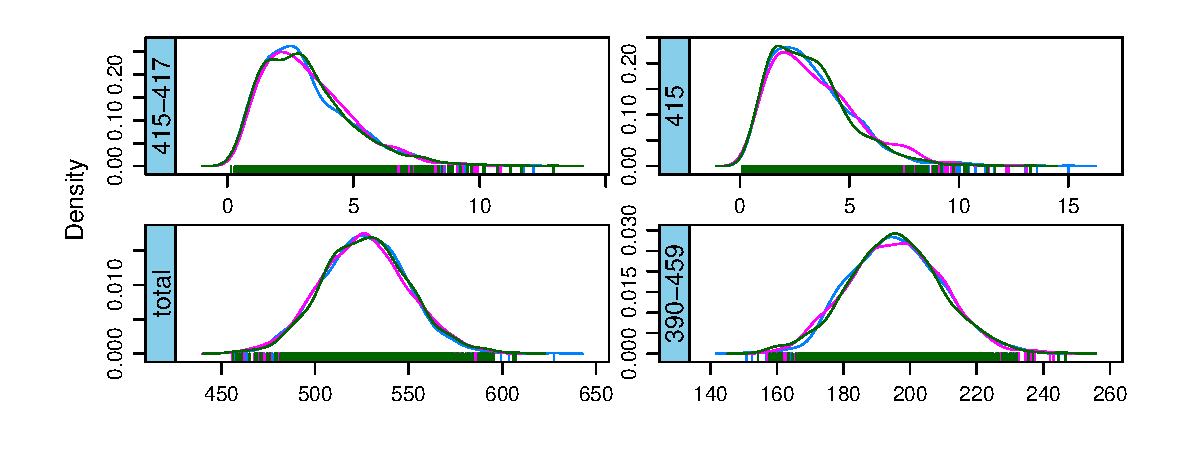
\includegraphics[width=1\linewidth]{../../R-codes/JAGS/plots/mimic/Density415h}
	\caption{Posterior distributions for ICD 452 and its ancestors, with added anomalies, and calculated with Hierarchical Bayes model}
	\label{fig:density452h}
\end{figure}

Table~\ref{tab:postsum452.mimic} and figure~\ref{fig:density452} shows the posterior for IBM and table~\ref{tab:postsum452h.mimic} and figure~\ref{fig:density452h} shows the posterior for HBM, for ICD 452 and its ancestors, with added anomalies. There are no obvious differences between the distribution values and distribution shape for IBM and HBM.

\newpage %----------------------------- all ----------------------------------    

\begin{figure}[!h]
	\centering
	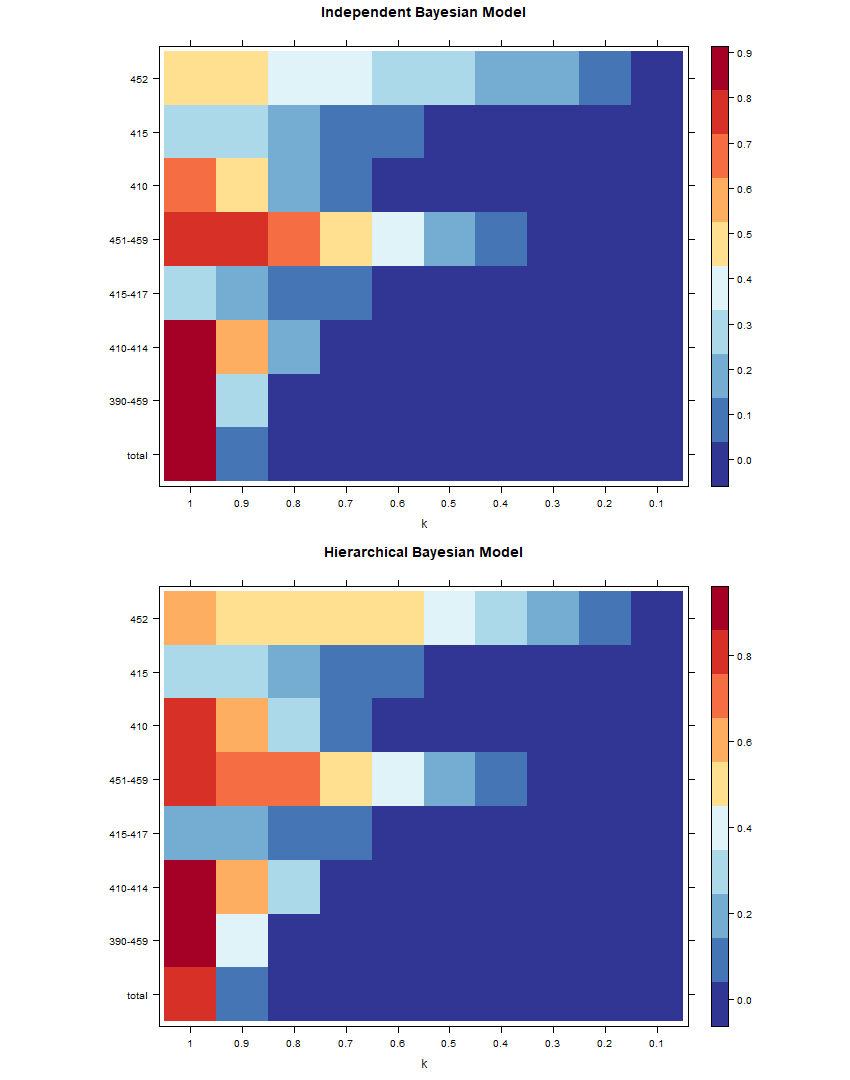
\includegraphics[width=1\linewidth]{../../R-codes/JAGS/plots/mimic/heatnorm}
	\caption{Heat-map of anomaly signals for ICD 410,415 and 452 and its ancestors, with no added anomalies, of IBM and HBM.}
	\label{fig:heatnorm}
\end{figure}

\newpage

\begin{figure}[!h]
	\centering
	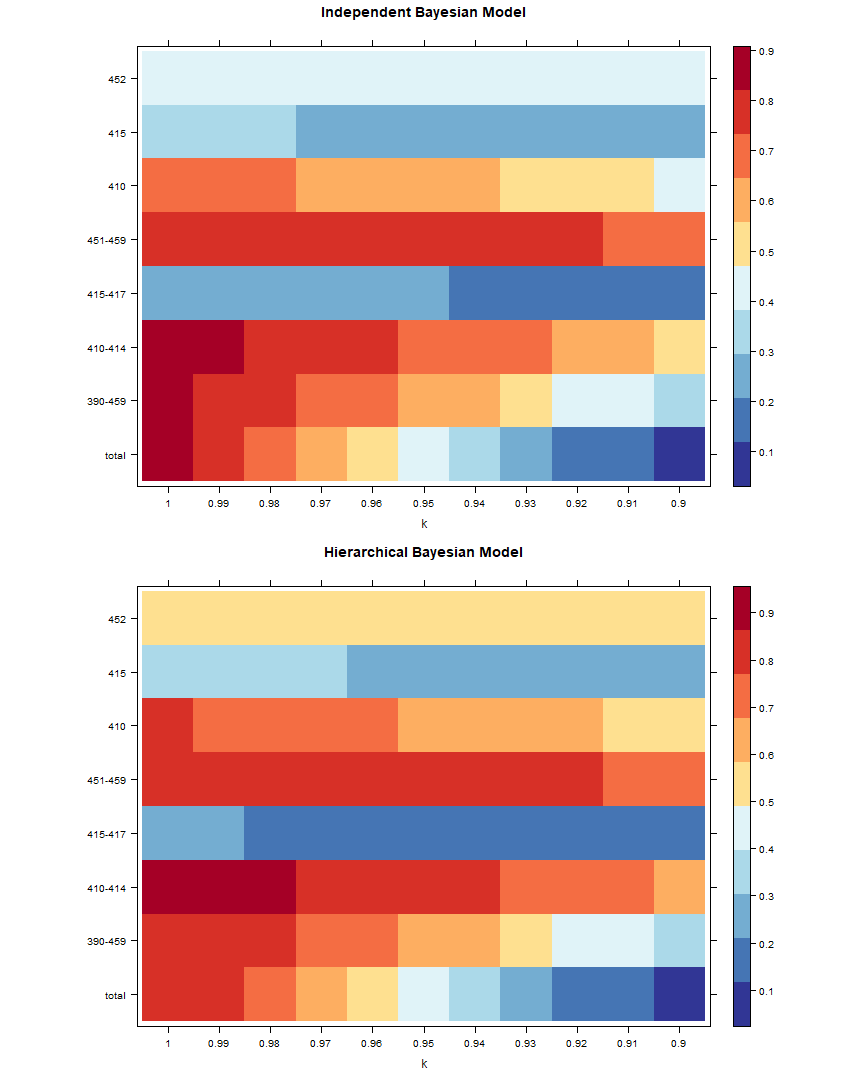
\includegraphics[width=1\linewidth]{../../R-codes/JAGS/plots/mimic/heatnorm2}
	\caption{Heat-map of anomaly signals for ICD 410,415 and 452 and their ancestors, with no added anomalies, of IBM and HBM zoomed in at k values of 0.9 to 1.}
	\label{fig:heatnorm2}
\end{figure}

\newpage

The heat-map in figure~\ref{fig:heatnorm} presents the anomaly signals of ICD 410,415 and 452 and their ancestors with no addition of a constant anomaly, with IBM and HBM, against different increments of $k$.Anomaly signals tend to be stronger as k increase, and stronger for lower hierarchies compare to higher hierarchies, the variability of signal strength also tend to increase with higher hierarchy. Zooming in at looking at k values from 0.6 to 1 in figure~\ref{fig:heatnorm2}, we observe a noticeable small difference in anomaly detection rate between IBM and HBM for category AA. Our observation suggests that the difference between anomaly detection rate is small or close to none for IBM and HBM, on the bottom of the hierarchy, for anomaly with a different hierarchical structure, in a simulated setting with each category generated independently.   

\newpage%----------------------------- 410 ----------------------------------

\begin{figure}[!h]
	\centering
	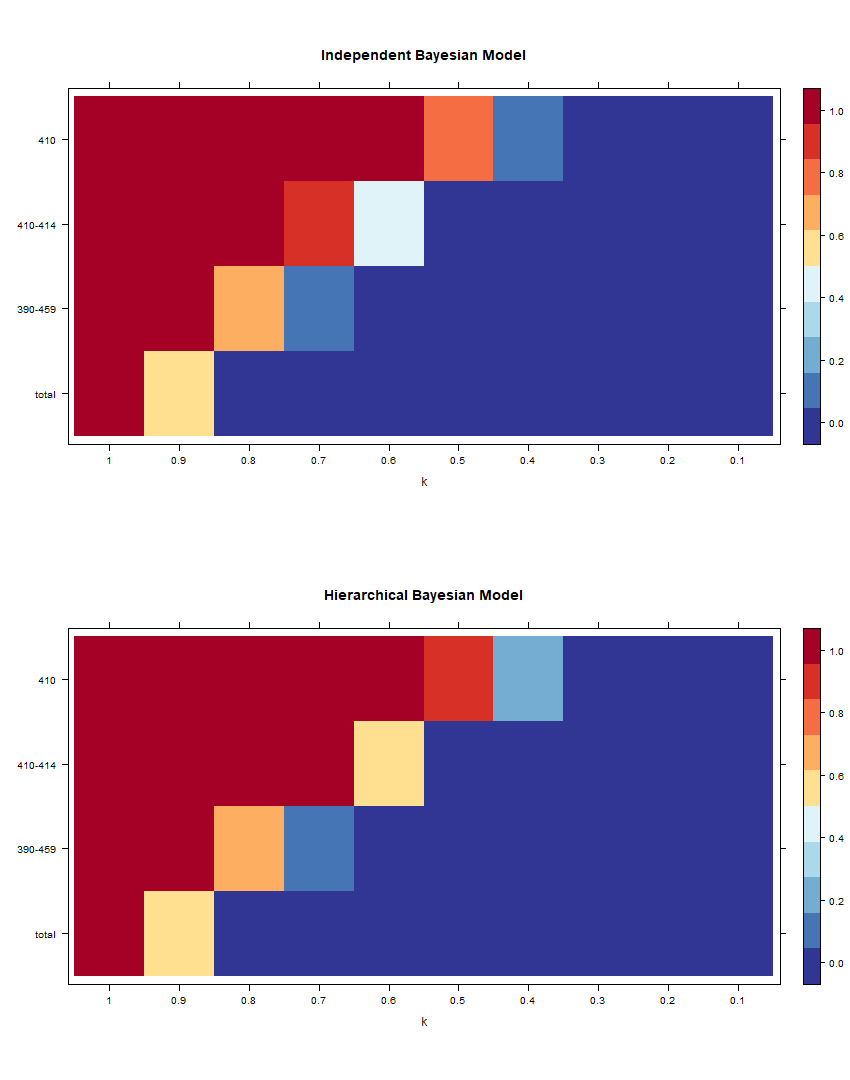
\includegraphics[width=1\linewidth]{../../R-codes/JAGS/plots/mimic/heat410}
	\caption{Heat-map of anomaly signals for ICD 410 and its ancestors, with no added anomalies, of IBM and HBM.}
	\label{fig:heat410}
\end{figure}

\newpage

\begin{figure}[!h]
	\centering
	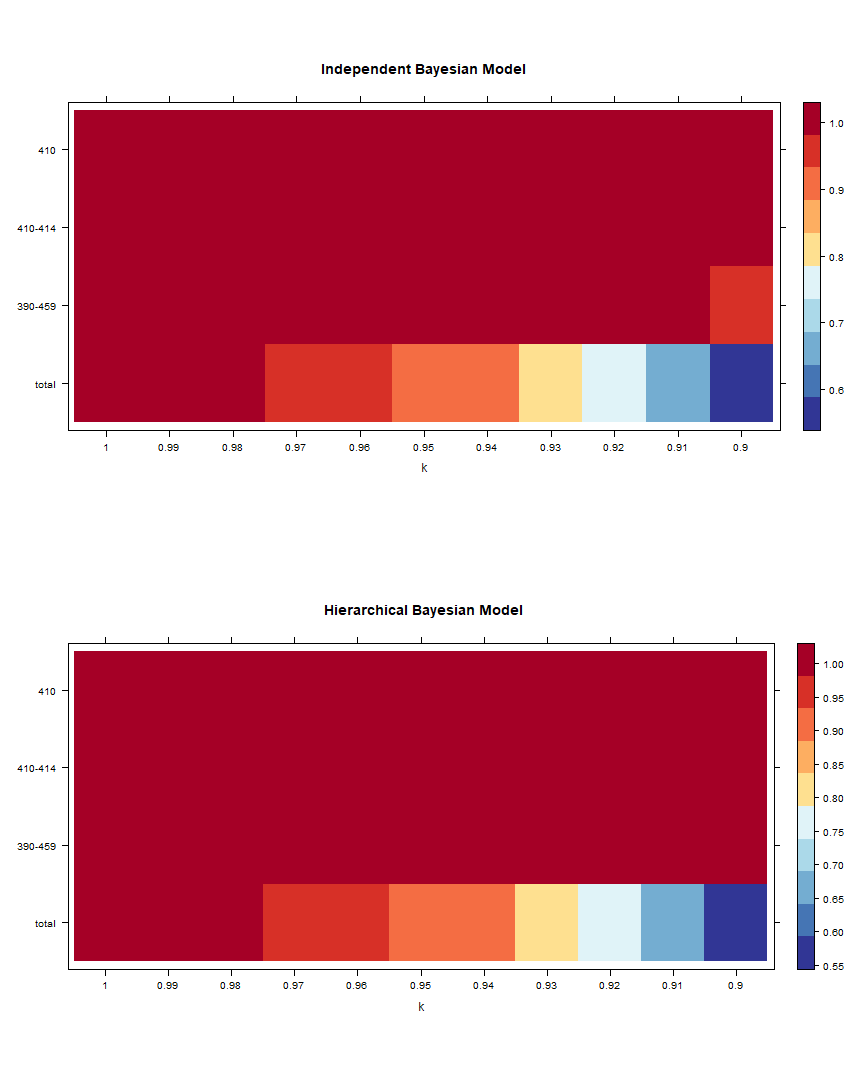
\includegraphics[width=1\linewidth]{../../R-codes/JAGS/plots/mimic/heat4102}
	\caption{Heat-map of anomaly signals for ICD 410 and its ancestors, with no added anomalies, of IBM and HBM zoomed in at k values of 0.9 to 1.}
	\label{fig:heat4102}
\end{figure}

\newpage

The heat-map in figure~\ref{fig:heat410} presents the anomaly signals of ICD 410 and their ancestors with no addition of a constant anomaly, with IBM and HBM, against different increments of $k$.Anomaly signals tend to be strong on the top left of the heat map. This suggests that signals of anomaly tend to increase in strength with increased k and higher hierarchy. Zooming in at looking at k values from 0.6 to 1 in figure~\ref{fig:heat4102}, we observe a noticeable small difference in anomaly detection rate between IBM and HBM for category AA. Our observation suggests that the difference between anomaly detection rate is small or close to none for IBM and HBM, on the bottom of the hierarchy, for anomaly with a different hierarchical structure, in a simulated setting with each category generated independently. 

\newpage%----------------------------- 415 ----------------------------------

\begin{figure}[!h]
	\centering
	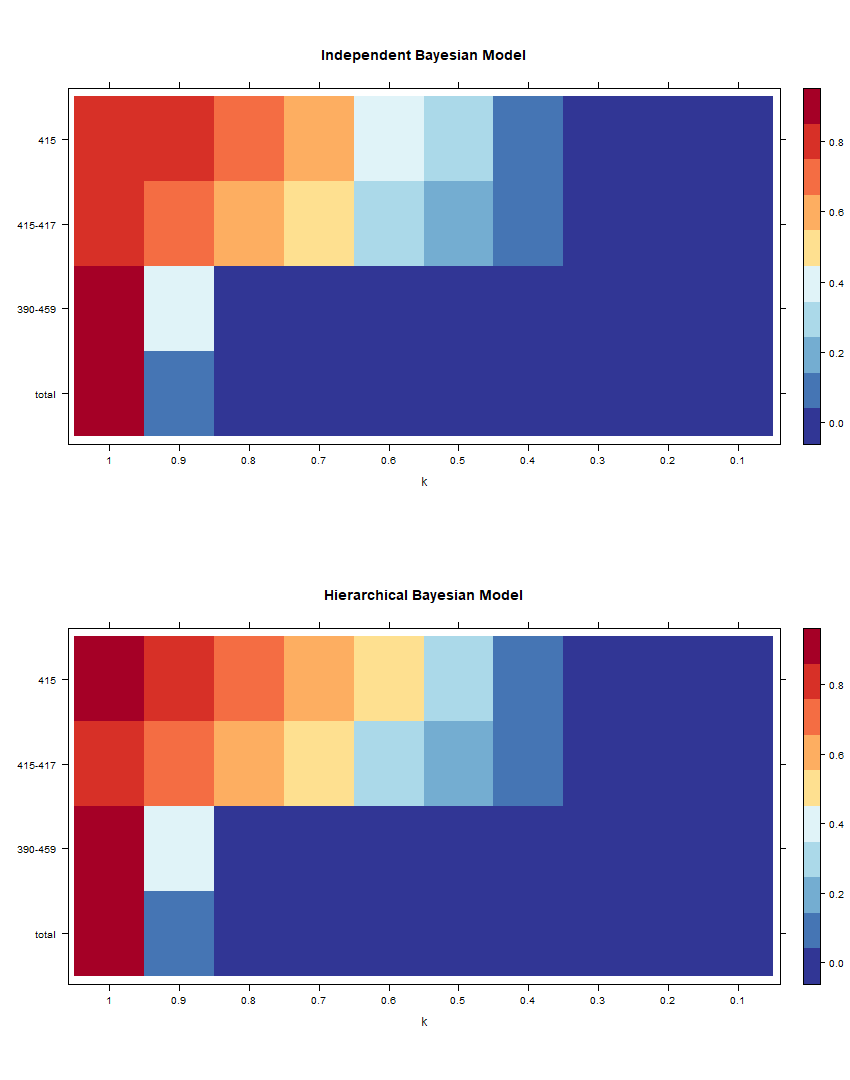
\includegraphics[width=1\linewidth]{../../R-codes/JAGS/plots/mimic/heat415}
	\caption{Heat-map of anomaly signals for ICD 415 and its ancestors, with no added anomalies, of IBM and HBM.}
	\label{fig:heat415}
\end{figure}

\newpage

\begin{figure}[!h]
	\centering
	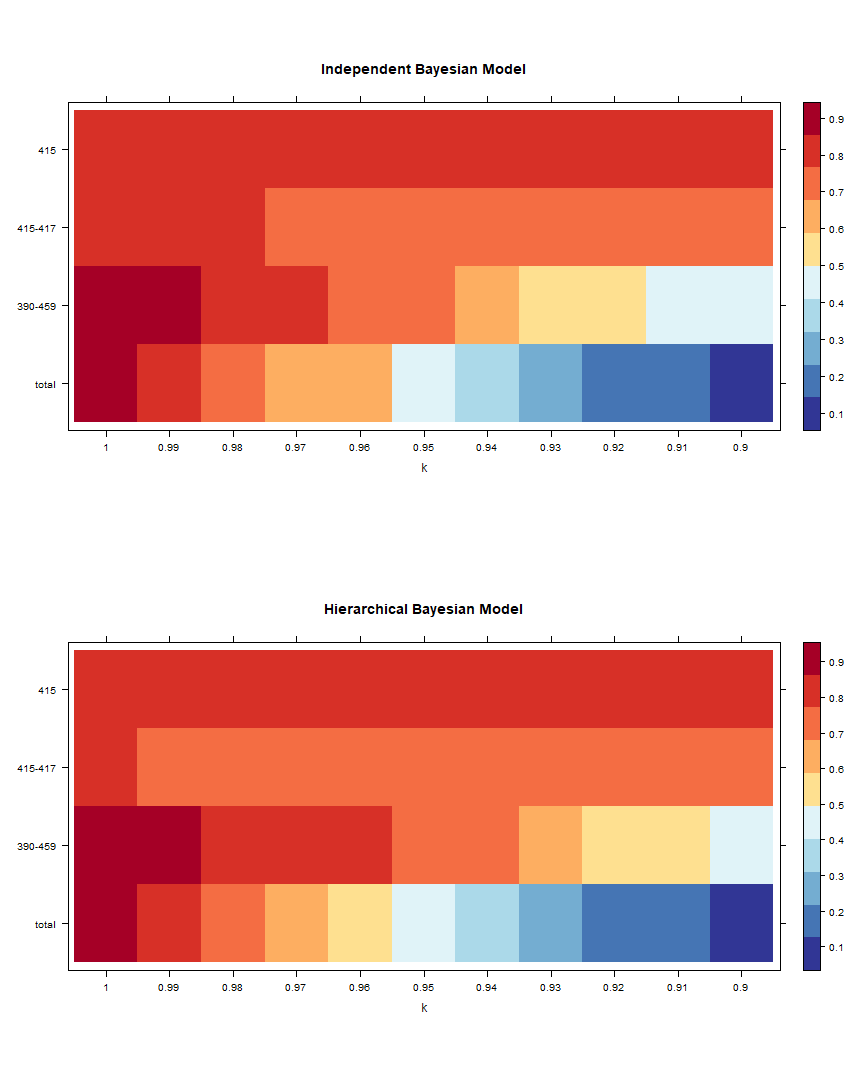
\includegraphics[width=1\linewidth]{../../R-codes/JAGS/plots/mimic/heat4152}
	\caption{Heat-map of anomaly signals for ICD 415 and its ancestors, with no added anomalies, of IBM and HBM zoomed in at k values of 0.9 to 1.}
	\label{fig:heat4152}
\end{figure}

\newpage

The heat-map in figure~\ref{fig:heat415} presents the anomaly signals of ICD 415 and their ancestors with no addition of a constant anomaly, with IBM and HBM, against different increments of $k$.Anomaly signals tend to be strong on the top left of the heat map. This suggests that signals of anomaly tend to increase in strength with increased k and higher hierarchy. Zooming in at looking at k values from 0.6 to 1 in figure~\ref{fig:heat4152}, we observe a noticeable small difference in anomaly detection rate between IBM and HBM for category AA. Our observation suggests that the difference between anomaly detection rate is small or close to none for IBM and HBM, on the bottom of the hierarchy, for anomaly with a different hierarchical structure, in a simulated setting with each category generated independently.

\newpage%----------------------------- 452 ----------------------------------

\begin{figure}[!h]
	\centering
	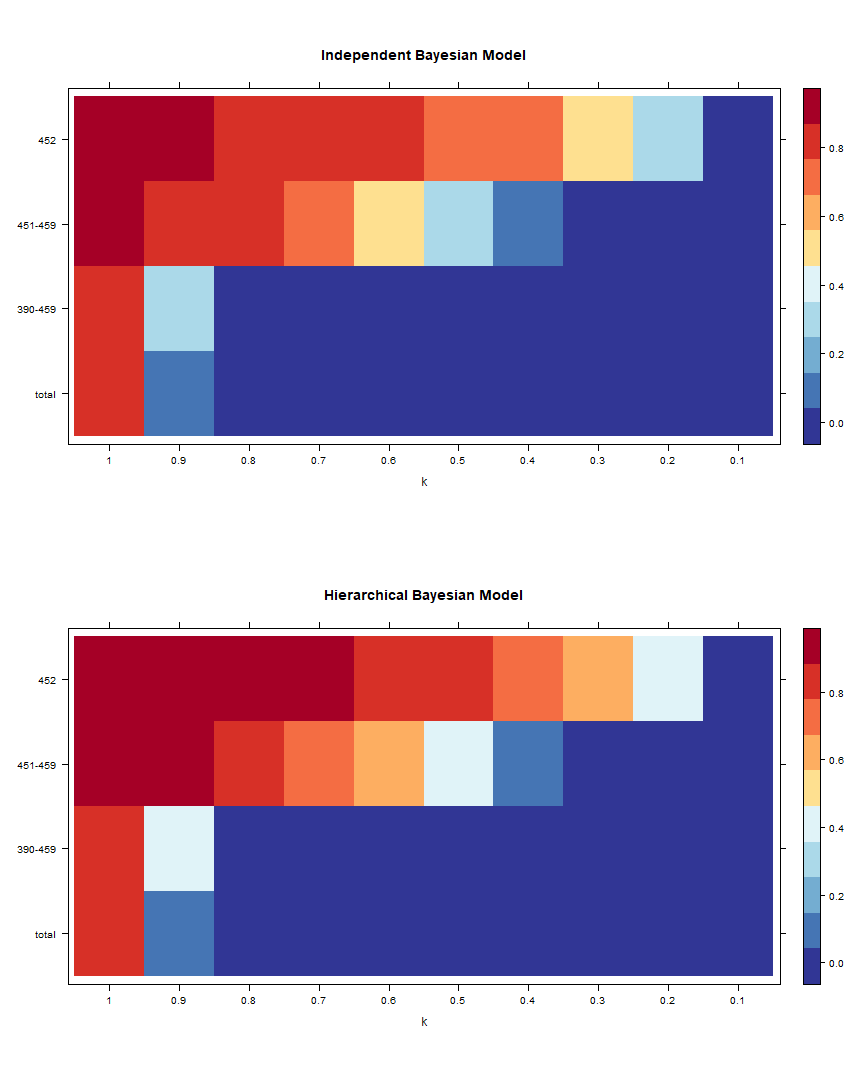
\includegraphics[width=1\linewidth]{../../R-codes/JAGS/plots/mimic/heat452}
	\caption{Heat-map of anomaly signals for ICD 452 and its ancestors, with no added anomalies, of IBM and HBM.}
	\label{fig:heat452}
\end{figure}

\newpage

\begin{figure}[!h]
	\centering
	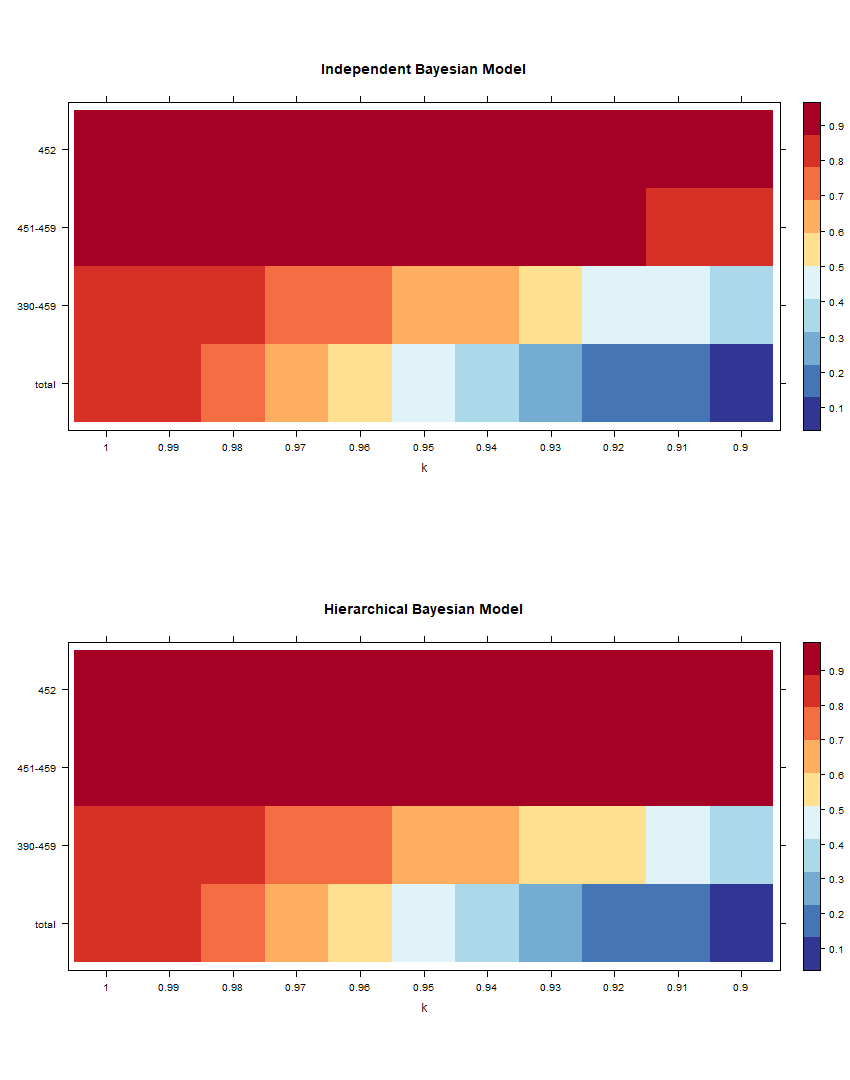
\includegraphics[width=1\linewidth]{../../R-codes/JAGS/plots/mimic/heat4522}
	\caption{Heat-map of anomaly signals for ICD 452 and its ancestors, with no added anomalies, of IBM and HBM zoomed in at k values of 0.9 to 1.}
	\label{fig:heat4522}
\end{figure}

\newpage

The heat-map in figure~\ref{fig:heat452} presents the anomaly signals of ICD  452 and their ancestors with no addition of a constant anomaly, with IBM and HBM, against different increments of $k$. Anomaly signals tend to be strong on the top left of the heat map. This suggests that signals of anomaly tend to increase in strength with increased k and higher hierarchy. Zooming in at looking at k values from 0.6 to 1 in figure~\ref{fig:heat4522}, we observe a noticeable small difference in anomaly detection rate between IBM and HBM for category AA. Our observation suggests that the difference between anomaly detection rate is small or close to none for IBM and HBM, on the bottom of the hierarchy, for anomaly with a different hierarchical structure, in a simulated setting with each category generated independently.

\newpara

There are significant differences in anomaly signals of disease categories with different rate of occurrence. For common diseases (ICD 410)the signals seem to be more clear (change in colour for different increments of $k$ is more abrupt) compare to rare (ICD 415) and extremely rare (ICD 452)disease categories. Signals seem to exist for categories at level 3 readily and level 2 of the hierarchy, for commonly diseases signals can be observed in level 1, but for rare and extremely rare diseases there is almost no signal at level 1. Signals at level 2 seem to be weaker than signals at level 3 overall, but it is still apparent and easily detectable.  

\section{Discussion}

We were unable to make a conclusion for the goodness-of-fit comparison between IBM and HBM because the mean and median values of differences in DIC are very close to 0. This suggests that for real-life data with large complex hierarchical structures, IBM and HBM performed very similarly. The finding is unexpected, as our simulation studies and several academic papers all seem to have suggested HBM be the superior model. There are several possible explanations for this. The first explanation is that for large complex hierarchical structures there are a huge amount of categories at each of the levels, and randomness from all these categories could have masked the small improvements in the goodness of fit for anomalies at one small category. Also that our HBM are quite primitive and there is no way for us to know whether or it really captures the hierarchical relationship, and the validity of our HBM is in question. If our HBM does not capture the hierarchical structure information, then there will not be any reason that HBM performs IBM. We also made observations that, for an extremely rare disease, the posterior distribution is not normal an seem to be skewed, but our model assumes it to be normal. We could possibly use different priors for categories with different magnitude of counts, for example, assigning a Half-Cauchy prior that was suggested by \citet{gelman2006prior} for extremely rare categories. 

\newpara

The mean of posterior distribution of disease with different prevalence of occurrence using IBM and HBM yield significant differences, with IBM yielding larger mean. For common disease the difference at leaf level is large, less common the less the difference, with uncommon disease there are almost no noticeable difference. This happens because for IBM, there are no information about the hierarchical structure that constraint the convergence in the MCMC process, thus a single abnormal observation have a greater influence on the posterior. And for HBM, the hierarchical structure meant that we are considering more than just the leaf level, but other higher levels as well.  

\newpara

There are significant differences in anomaly signals of disease categories with different rate of occurrence. We noticed that for common disease category signals of the anomaly are still visible at level 1 of the hierarchy, but for rare and extremely are disease categories, there is almost no signal. However, signals can still be readily observed at level 2 and level 3 of the hierarchy for rare and extremely rare disease categories. Our observation made sense because rare and common disease have a much smaller magnitude of counts and as lower hierarchy aggregate into a higher hierarchy, smaller counts tend to get masked by randomness and uncertainty from other categories, so it would become harder to detect the anomaly at higher hierarchy levels. For ICD-9 disease categories, we are able to detect anomaly at the bottom two levels. This suggests that we should not look at anomaly at level 1 of hierarchy because we are likely to miss it. The rarity of disease also have a significant impact on anomaly detection, for common disease with large average values, signals of the anomaly are clear and easy to detect, but for rare and extremely rare disease categories it is unclear and harder to decide.

\newpara

Overall we see that if the capacity is under 60\% ish, there are almost no anomaly signal, this meant that if the hospitals are operating at capacities at or under 60\%, they will almost never exceed their full capacity even if there are twice as many arrivals for certain disease categories compare to usual. It is a bit hard to make sense of this, but essentially what you need to know is that operating at a lower capacity should have a significant impact on the likelihood of anomalous arrivals. The obvious solution to congestion is to decrease the operation capacity (or increase overall capacity), but this is easier said than been done because the hospitals would have done it if they could. However, our results still high lighted the fact that having a lower operation capacity could effectively buffer against anomalous events and reduce the likelihood of congestion from occurring. 
	
	
